\begin{figure}
\centering
\begin{minipage}{0.14\textwidth}
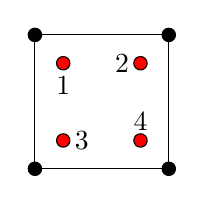
\begin{tikzpicture}[scale=0.85]
\draw[step=2 cm] (0,0) grid (2,2);
\foreach \y in {0,2}{
\draw [fill=black](0,\y) circle (0.1cm);
\draw [fill=black](2,\y) circle (0.1cm);
}
% \foreach \y in {0.2115, 0.7885}{
% 	\draw [fill=black](0.2115,\y) circle (0.1cm);
% 	\draw [fill=black](0.7885,\y) circle (0.1cm);
% }
\foreach \y in {0.423, 1.577}{
\draw [fill=red](0.423,\y) circle (0.1cm);
\draw [fill=red](1.577,\y) circle (0.1cm);
}
\draw (0.423, 1.25) node {1};
\draw (1.3,1.577) node {2};
\draw (0.7, 0.423) node {3};
\draw (1.577, 0.7) node {4};
\end{tikzpicture}
\end{minipage}
\begin{minipage}{0.35\textwidth}
\centering
\begin{tikzpicture}[scale=0.85]
\newcommand\reclenH{3}
\newcommand\reclenV{4}
\newcommand\ndiv{4}
\newcommand\stepsize{1}
\newcommand\xl{0}
\newcommand\yl{0}
\newcommand\osx{-0.5}
\newcommand\osy{0.5}
%		\fill[cpu2] (\xl,\yl) rectangle (\xl+\reclenH,\yl+\reclenV);
\draw[step=\stepsize cm] (\xl,\yl) grid (\xl+\reclenH,\yl+\reclenV);
%	\draw (0, 0) node {$test$};

\foreach \y in {0,1,2,3,4}{
\draw [fill=black](0,\y) circle (0.1cm);
\draw [fill=black](1,\y) circle (0.1cm);
\draw [fill=black](2,\y) circle (0.1cm);
\draw [fill=black](3,\y) circle (0.1cm);
}

\draw (\osx, 0) node {$e$};
\draw (\osx, 1) node {$d$};
\draw (\osx, 2) node {$c$};
\draw (\osx, 3) node {$b$};
\draw (\osx, 4) node {$a$};

\draw (0,\reclenV + \osy) node {$1$};
\draw (1,\reclenV + \osy) node {$2$};
\draw (2,\reclenV + \osy) node {$3$};
\draw (3,\reclenV + \osy) node {$4$};

\foreach \y in {0.2115, 0.7885, 1.2115, 1.7885, 2.2115, 2.7885, 3.2115, 3.7885}{
\draw [fill=red](0.2115,\y) circle (0.08cm);
\draw [fill=red](0.7885,\y) circle (0.08cm);
\draw [fill=red](1.2115,\y) circle (0.08cm);
\draw [fill=red](1.7885,\y) circle (0.08cm);
\draw [fill=red](2.2115,\y) circle (0.08cm);
\draw [fill=red](2.7885,\y) circle (0.08cm);
}

\foreach \y in {0.7885, 1.7885, 2.7885, 3.7885}{
\draw [fill=green](0.2115,\y) circle (0.08cm);
\draw [fill=green](1.2115,\y) circle (0.08cm);
\draw [fill=green](2.2115,\y) circle (0.08cm);
% \draw [fill=green](0.7885,\y) circle (0.08cm);
% \draw [fill=green](1.7885,\y) circle (0.08cm);
% \draw [fill=green](2.7885,\y) circle (0.08cm);
}

\end{tikzpicture}		
\end{minipage}	
\caption {(Left) A single 2D element in FEM, with black dots denoting ``nodes" and red dots denoting $ 2\times 2 $ Gauss quadrature points. (Right) A finite element mesh, with $ 4\times 3 $ linear elements and $ 5\times 4 $ nodes. Each of these elements contains Gauss points for integration to be performed within that element. Within each element, the ``first" quadrature point (marked ``1" on left) is marked green, and others red.}
\label{fig:fem-mesh-with-gauss-pt}
\end{figure}
																							
\begin{figure}[!htb]
\centering
\begin{tikzpicture}
% ------- style -------
\tikzset{%
parenthesized/.style={%
left delimiter  = (,
right delimiter = ),
},
node distance = 5mu,
}

% ------- equation -------		

\matrix[matrix of math nodes, parenthesized] (I) {
a_1 & a_2 & a_3 & a_4 \\
b_1 & b_2 & b_3 & b_4 \\
c_1 & c_2 & c_3 & c_4 \\
d_1 & d_2 & d_3 & d_4 \\
e_1 & e_2 & e_3 & e_4 \\
};
%	\color{black}
\node (*) [right = of I] {${}*{}$};

%	\matrix[matrix of math nodes, parenthesized] (K) [right = of *] {
%		0 & \frac{1}{h^2} & 0 \\
%		\frac{1}{h^2} & \frac{-4}{h^2} & \frac{1}{h^2} \\
%		0 & \frac{1}{h^2} & 0 \\
%	};
\matrix[matrix of math nodes, parenthesized] (K) [right = of *] {
N_1 & N_2 \\
N_3 & N_4 \\
};

\node (=) [right = of K] {${}={}$};

% \matrix[matrix of math nodes, parenthesized] (I*K) [right = of {=}] {
% 	z_1 & z_2\\
% 	z_3 & z_4\\
% 	z_5 & z_6\\
% };
\matrix[matrix of math nodes, parenthesized] (I*K) [right = of {=}] {
\color{green}\bullet & \color{green}\bullet & \color{green}\bullet\\
\color{green}\bullet & \color{green}\bullet & \color{green}\bullet\\
\color{green}\bullet & \color{green}\bullet & \color{green}\bullet\\
\color{green}\bullet & \color{green}\bullet & \color{green}\bullet\\
};
% ------- highlighting -------
\newcommand\rowResult{2}
\newcommand\colResult{1}

\begin{scope}[on background layer]
\newcommand{\padding}{2pt}
\coordinate (Is-nw) at ([xshift=-\padding, yshift=+\padding] I-\rowResult-\colResult.north west);
\coordinate (Is-se) at ([xshift=+\padding, yshift=-\padding] I-\the\numexpr\rowResult+\numRowsK-2\relax-\the\numexpr\colResult+\numColsK-2\relax.south east);
\coordinate (Is-sw) at (Is-nw |- Is-se);
\coordinate (Is-ne) at (Is-se |- Is-nw);

\filldraw[red,   fill opacity=.1] (Is-nw) rectangle (Is-se);
\filldraw[green, fill opacity=.1] (I*K-\rowResult-\colResult.north west) rectangle (I*K-\rowResult-\colResult.south east);

\draw[blue, dotted] 
(Is-nw) -- (K.north west)
(Is-se) -- (K.south east)
(Is-sw) -- (K.south west)
(Is-ne) -- (K.north east)
;
\draw[green, dotted] 
(I*K-\rowResult-\colResult.north west) -- (K.north west)
(I*K-\rowResult-\colResult.south east) -- (K.south east)
(I*K-\rowResult-\colResult.south west) -- (K.south west)
(I*K-\rowResult-\colResult.north east) -- (K.north east)
;

\draw[blue,  fill=blue!10!white] (K.north west) rectangle (K.south east);
\end{scope}

% ------- labels -------
\tikzset{node distance=0em}
\node[below=of I] (I-label) {$ (U^d_\theta)_M $};
\node at (K |- I-label)     {$ K_{GP1} $};
\node at (I*K |- I-label)   {$ ((U^d_\theta)_{GP_1})_M $};
\end{tikzpicture}%
\caption{Quadrature quantity evaluation in FEM context. $ (U^d_\theta)_M $ is the matrix view of the nodal values.$ K_{GP1} $ is kernel containing the basis function values at ``gauss point - 1" (top left corner). This convolution results in the function values evaluated at the Gauss point ``1" of each element (marked green). $ (U^d_\theta{}_{GP1})_M $ is the matrix of this result. Function values (or their derivatives) evaluated at Gauss  points can then be used in any integral evaluation. For example, $ \int u^h dD = |J| \sum_{I\in M} \left[\sum_{i=1}^{4}(w_i (U^d_\theta)_{GPi})_M\right] $, where $ |J| $ is the transformation Jacobian for integration and $ w $ are the quadrature weights.}
\label{fig:fem-function-evaluation-at-single-gauss-pt}
\end{figure}